\begin{figure}[h]
	\centering
	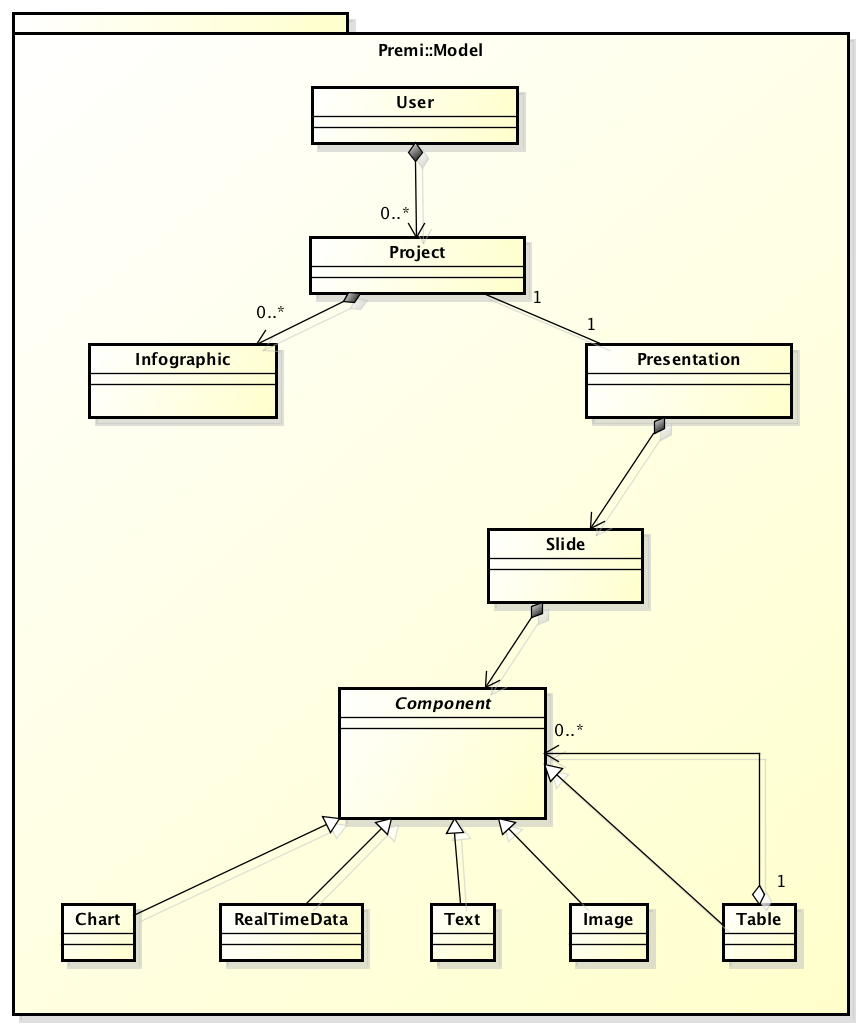
\includegraphics[width=0.7\linewidth]{img/premi_model}
	\caption[Premi::Front-End::Model]{Premi::Front-End::Model}
\end{figure}
Il package gestisce la memorizzazione delle informazioni dei dati utilizzati nel \gls{front-end} e la loro logica. Al suo interno è presente una struttura di classi creata per ottimizzare il recupero e il salvataggio di dati anche con il rispettivo model del \gls{back-end}.\\
%Non è stato inserito un dettaglio di metodi ed attributi per quanto riguarda il \gls{front-end} poiché è stato mantenuto identico a quello del \gls{back-end} e si sarebbe trattata di una ridondanza che non avrebbe portato nessuna informazione aggiuntiva.


\newpage


\subsubsection{User}

	\begin{figure}[h]
		\centering
		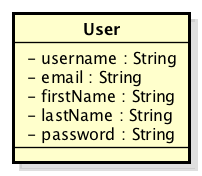
\includegraphics[width=0.4\linewidth]{img/premi_front_end_model_user}
		\caption[Diagramma della classe User]{Diagramma della classe User}
	\end{figure}
	
	\paragraph{Descrizione:}
	Il modello User permette di gestire la collezione users del \gls{database}, relativa agli utenti registrati.
	
	\paragraph{Utilizzo:}
	La classe modella la collezione users del \gls{database}.
	
	\paragraph{Attributi:}
		\begin{itemize}
			\item \textbf{- username: String}:\\
				Contiene il nome utente scelto dall'utente;
			\item \textbf{- email: String}:\\
				Contiene l'indirizzo email inserito dall'utente;
			\item \textbf{- firstName: String}:\\
				Contiene il nome inserito dall'utente;
			\item \textbf{- lastName: String}:\\
				Contiene il cognome inserito dall'utente;
			\item \textbf{- password: String}:\\
				Contiene la password scelta dall'utente.
		\end{itemize}


\newpage


\subsubsection{Project}

	\begin{figure}[h]
		\centering
		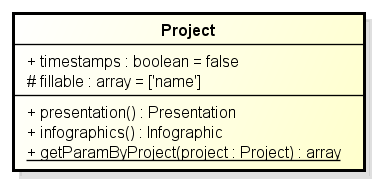
\includegraphics[width=0.4\linewidth]{img/back_end_premi_model_project}
		\caption[Diagramma della classe Project]{Diagramma della classe Project}
		\label{fig:back_end_premi_model_project}
	\end{figure}
	
	\paragraph{Descrizione:}
	Questa classe rappresenta un progetto di un utente.
	
	\paragraph{Utilizzo:}
	Viene utilizzata alla creazione di un progetto di un utente.
	
	\paragraph{Attributi:}
	\begin{itemize}
		\item \textbf{- name: String}:\\
			Campo dati contenente il nome del progetto.
	\end{itemize}


\newpage


\subsubsection{Infographic}

\begin{figure}[h]
	\centering
	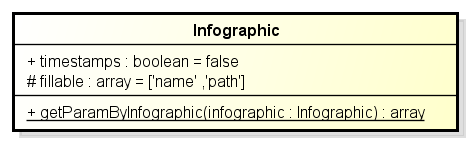
\includegraphics[width=0.4\linewidth]{img/back_end_premi_model_infographic}
	\caption[Diagramma della classe Infographic]{Diagramma della classe Infographic}
	\label{fig:back_end_premi_model_infographic}
\end{figure}
	
	\paragraph{Descrizione:}
	Questa classe rappresenta un'\gls{infografica} di un progetto, ovvero una rappresentazione visuale della presentazione per mostrare in maniera semplice e veloce le informazioni.
	
	\paragraph{Utilizzo:}
	Viene utilizzata alla creazione di un'\gls{infografica} di una progetto.
	
	\paragraph{Attributi:}
	\begin{itemize}
		\item \textbf{- name: String}:\\
			Campo dati contenente il nome dell'\gls{infografica};
		\item \textbf{- path: String}:\\
			Campo dati contenente il percorso dove recuperare il file dell'\gls{infografica}.
		\end{itemize}
			
	
\newpage


\subsubsection{Presentation}

	\begin{figure}[h]
		\centering
		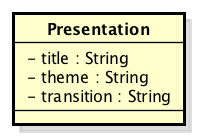
\includegraphics[width=0.4\linewidth]{img/premi_front_end_model_presentation}
		\caption[Diagramma della classe Presentation]{Diagramma della classe Presentation}
		\label{fig:back_end_premi_model_presentation}
	\end{figure}
	
	
	\paragraph{Descrizione:}
	Questa classe descrive la presentazione di un progetto. Contiene tutte le \textit{\gls{slide}} che servono a comporre la presentazione.
	
	\paragraph{Utilizzo}
	Viene utilizzato alla creazione o caricamento di una presentazione.
	
	\paragraph{Attributi:}
	\begin{itemize}
		\item \textbf{- title: String}:\\
			Campo dati contenente il titolo della presentazione;
		\item \textbf{- theme: String}:\\
			Campo dati contenente il tema, inteso come \textit{\gls{font}} e colore di sfondo, utilizzato per la presentazione;
		\item \textbf{- transition: String}:\\
			Campo dati contenente il tipo di transizione da una \textit{\gls{slide}} all'altra durante la visualizzazione della presentazione.
	\end{itemize}


\newpage


\subsubsection{Slide}

	\begin{figure}[h]
		\centering
		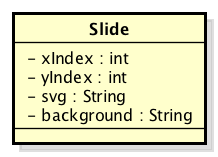
\includegraphics[width=0.4\linewidth]{img/premi_front_end_model_slide}
		\caption[Diagramma della classe \gls{Slide}]{Diagramma della classe Slide}
		\label{fig:back_end_premi_model_slide}
	\end{figure}
	
	
	\paragraph{Descrizione:}
	Questa classe descrive una singola \gls{slide}. Contiene tutti i gli oggetti appartenenti alla \gls{slide}.
	
	\paragraph{Utilizzo:}
	Viene utilizzato alla creazione o caricamento di una \gls{slide}.
	
	\paragraph{Attributi:}
	\begin{itemize}
		\item \textbf{- xIndex: int}:\\
			Campo dati contenente la posizione relativa all'asse X delle \gls{slide} nella matrice di \gls{slide} della presentazione;
		\item \textbf{- yIndex: int}:\\
			Campo dati contenente la posizione relativa all'asse Y delle \gls{slide} nella matrice di \gls{slide} della presentazione;
		\item \textbf{- svg: String}:\\
			Campo dati contenente la stringa SVG relativa alla \gls{slide};
		\item \textbf{- background: String}:\\
			Campo dati contenente il colore di sfondo di una \gls{slide}.
	\end{itemize}
	
	
\newpage


\subsubsection{Component}

	\begin{figure}[h]
		\centering
		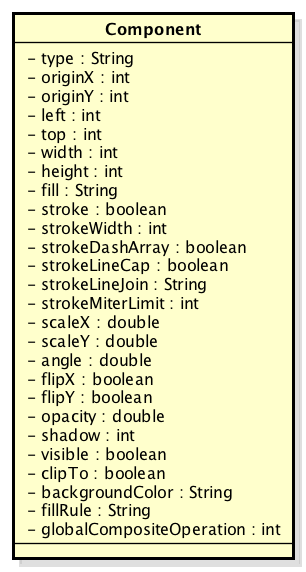
\includegraphics[width=0.4\linewidth]{img/premi_front_end_model_component}
		\caption[Diagramma della classe Component]{Diagramma della classe Component}
		\label{fig:back_end_premi_model_component}
	\end{figure}
	
	
	\paragraph{Descrizione:}
	Questa classe descrive la struttura generica di un componente.
	
	\paragraph{Utilizzo:}
	Viene utilizzato alla creazione o caricamento di una componente.
	
	\paragraph{Attributi:}
	\begin{itemize}
		\item \textbf{- type: String}:\\
			Campo dati contenente il tipo di componente;
		\item \textbf{- originX: int}:\\
			Campo dati contenente la posizione relativa all'asse X del vertice d'origine del componente;
		\item \textbf{- originY: int}:\\
			Campo dati contenente la posizione relativa all'asse Y del vertice d'origine del componente;
		\item \textbf{- left: int}:\\
			Campo dati contenente la posizione relativa all'asse delle X dell'area di disegno in cui verrà disegnato il componente;
		\item \textbf{- top: int}:\\
			Campo dati contenente la posizione relativa all'asse delle Y dell'area di disegno in cui verrà disegna il componente;
		\item \textbf{- width: int}:\\
			Campo dati contenente larghezza del riquadro che racchiude il componente;
		\item \textbf{- height: int}:\\
			Campo dati contenente altezza del riquadro che racchiude il componente;
		\item \textbf{- fill: String}:\\
			Campo dati contenente il colore di riempimento del riquadro che racchiude il componente;
		\item \textbf{- stroke: boolean}:\\
			Campo dati contenente il colore del tratto utilizzato per disegnare il componente;
		\item \textbf{- strokeWidth: int}:\\
			Campo dati contenente la larghezza del tratto utilizzato per disegnare il componente;
		\item \textbf{- strokeDashArray: boolean}:\\
			Campo dati contenente il tipo di tratto utilizzato per disegnare il componente;
		\item \textbf{- strokeLineCap: boolean}:\\
			Campo dati contenente lo stile di fine del tratto utilizzato per disegnare il componente;
		\item \textbf{- strokeLineJoin:  String}:\\
			Campo dati contenente lo stile degli angoli del tratto utilizzato per disegnare il componente;
		\item \textbf{- strokeMiterLimit: int}:\\
			Campo dati contenente il limite della distanza di unione tra due linee;
		\item \textbf{- scaleX: double}:\\
			Campo dati contenente il valore con cui viene scalato in larghezza il componente;
		\item \textbf{- scaleY: double}:\\
			Campo dati contenente il valore con cui viene scalato in altezza il componente;
		\item \textbf{- angle: double}:\\
			Indica l'angolo di rotazione del componente;
		\item \textbf{- flipX: boolean}:\\
			Indica se il componente è capovolto rispetto all'asse X;
		\item \textbf{- flipY: boolean}:\\
			Indica se il componente è capovolto rispetto all'asse Y;
		\item \textbf{- opacity: double}:\\
			Campo dati contenente il livello di opacità del componente;
		\item \textbf{- shadow: int}:\\
			Campo dati contenente il livello dell'ombra del componente;
		\item \textbf{- visible: boolean}:\\
			Indica  se il componente è visibile o no;
		\item \textbf{- clipTo: boolean}:\\
			Indica se il componente ha l'effetto clip attivo;
		\item \textbf{- backgroundColor: String}:\\
			Campo dati contenente il colore di sfondo del componente;
		\item \textbf{- fillRule: String}:\\
			Campo dati contenente lo stile di riempimento;
		\item \textbf{- globalCompositeOperation: int}:\\
			Campo dati contenente l'ordine in cui vengono disegnati i componenti all'interno di un gruppo.
	\end{itemize}
	
	
\newpage


\subsubsection{Chart}

	\begin{figure}[h]
		\centering
		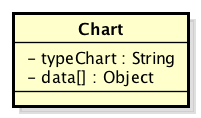
\includegraphics[width=0.4\linewidth]{img/premi_front_end_model_chart}
		\caption[Diagramma della classe Chart]{Diagramma della classe Chart}
		\label{fig:back_end_premi_model_chart}
	\end{figure}
	
	\paragraph{Descrizione}
	Questa classe rappresenta la struttura di dati necessari per descrivere un grafico all'interno di una \gls{slide}. Tale classe estende la classe Component.
	
	\paragraph{Utilizzo}
	Viene utilizzato alla creazione o caricamento di un grafico.
	
	\paragraph{Attributi}
	\begin{itemize}
		\item \textbf{- typeChart: String}:\\
			Campo dati che contiene il tipo di grafico;
		\item \textbf{- data[]: Object}:\\
			Campo dati che contiene l'array di dati che servono a comporre il grafico.
	\end{itemize}


\newpage


\subsubsection{RealTimeData}

	\begin{figure}[h]
		\centering
		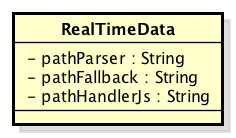
\includegraphics[width=0.4\linewidth]{img/premi_front_end_model_realtimedata}
		\caption[Diagramma della classe RealTimeData]{Diagramma della classe RealTimeData}
		\label{fig:back_end_premi_model_realTimeData}
	\end{figure}
	
	\paragraph{Descrizione}
	Questa classe rappresenta la struttura di dati necessari per descrivere RealTimeData (dato in tempo reale) all'interno di una \gls{slide}. Tale classe estende la classe Component.
	
	\paragraph{Utilizzo}
	Viene utilizzato alla creazione o caricamento di un RealTimeData.
	
	\paragraph{Attributi}
	\begin{itemize}
		\item \textbf{- pathParser: String}:\\
			Indirizzo del \gls{parser} \gls{php} \footnote{file \gls{php} con il compito di recuperare i dati da un indirizzo remoto (evitando cosi il problema della same-origin-policy) fornendo come risultato un oggetto \gls{JSON} che sarà poi processato dall'Handler \gls{javascript}};
		\item \textbf{- pathFallback: String}:\\
			Indirizzo del file contenente l'oggetto più recente salvato in caso di consultazione offline;
		\item \textbf{- pathHandlerJs: String}:\\
			Indirizzo del handler \gls{javascript} con il compito di impaginare i risultati provenienti dal \gls{parser} e ri aggiornare la vista dopo n secondi.
	\end{itemize}


\newpage


\subsubsection{Text}

	\begin{figure}[h]
		\centering
		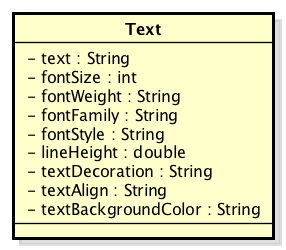
\includegraphics[width=0.4\linewidth]{img/premi_front_end_model_text}
		\caption[Diagramma della classe Text]{Diagramma della classe Text}
		\label{fig:back_end_premi_model_text}
	\end{figure}

	\paragraph{Descrizione}
	Questa classe rappresenta la struttura di dati di un campo di testo di una \gls{slide}. Tale classe estende la classe Component.
	
	\paragraph{Utilizzo}
	Viene utilizzato alla creazione o caricamento di un campo di testo.
	
	\paragraph{Attributi}
	\begin{itemize}
		\item \textbf{- text: String}:\\
			Campo dati contenente il contenuto del campo di testo;
		\item \textbf{- fontSize: int}:\\
			Campo dati contenente le dimensioni del \gls{font} del campo di testo;
		\item \textbf{- fontWeight: String}:\\
			Campo dati contenente lo spessore del testo;
		\item \textbf{- fontFamily: String}:\\
			Campo dati contenente la famiglia di \gls{font} del campo di testo;
		\item \textbf{- fontStyle: String}:\\
			Campo dati contenente lo stile del \gls{font} del campo di testo (corsivo, grassetto, sottolineato);
		\item \textbf{- lineHeight: double}:\\
			Campo dati contenente l'altezza della linea del campo di testo;
		\item \textbf{- textDecoration: String}:\\
			Campo dati contenente il tipo di decorazione;
		\item \textbf{- textAlign: String}:\\
			Campo dati contenente l'allineamento del testo all'interno del campo di testo;
		\item \textbf{- textBackgroundColor: String}:\\
			Campo dati contenente il colore di sfondo del campo di testo.
	\end{itemize}

\newpage


\subsubsection{Image}

	\begin{figure}[h]
		\centering
		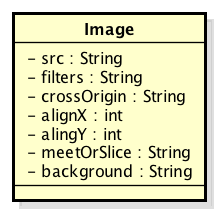
\includegraphics[width=0.4\linewidth]{img/premi_front_end_model_image}
		\caption[Diagramma della classe Image]{Diagramma della classe Image}
		\label{fig:back_end_premi_model_image}
	\end{figure}
	
	\paragraph{Descrizione}
	La classe Image rappresenta la struttura dei dati necessari per rappresentare un'immagine all'interno di una \gls{slide}. Tale classe estende la classe Component.
	
	\paragraph{Utilizzo}
	Utilizzata quando viene inserita un'immagine per tenerne traccia.
	
	\paragraph{Attributi}
	\begin{itemize}
		\item \textbf{- src: String}:\\
			Campo dati contenente il percorso dove recuperare il file dell'immagine;
		\item \textbf{- filters: String}:\\
			Campo dati contenente quali filtri verranno applicati all'immagine;
		\item \textbf{- crossOrigin: String}:\\
			Campo dati contenente utilizzato per passare informazioni assieme all'immagine;
		\item \textbf{- alignX: int}:\\
			Campo dati contenente l'allineamento relativo all'asse X dell'immagine;
		\item \textbf{- alignY: int}:\\
			Campo dati contenente l'allineamento relativo all'asse Y dell'immagine;
		\item \textbf{- meetOrSlice: String}:\\
			Indica se l'immagine dev'essere tagliata quando la sua finestra si restringe o essere sempre completamente visibile;
		\item \textbf{- background: String}:\\
			Campo dati contenente lo sfondo dell'immagine.
	\end{itemize}
	
	
\newpage


\subsubsection{Table}

	\begin{figure}[h]
		\centering
		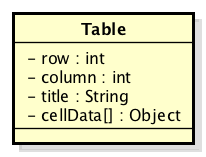
\includegraphics[width=0.4\linewidth]{img/premi_front_end_model_table}
		\caption[Diagramma della classe Table]{Diagramma della classe Table}
		\label{fig:back_end_premi_model_table}
	\end{figure}
	
	
	\paragraph{Descrizione}
	Questa classe rappresenta la struttura di dati di una tabella di una \gls{slide}. Tale classe estende la classe Component.
	
	\paragraph{Utilizzo}
	Viene utilizzato alla creazione o caricamento di una tabella.
	
	\paragraph{Attributi}
	\begin{itemize}
		\item \textbf{- row: int}:\\
			Campo dati contenente il numero di righe della tabella;
		\item \textbf{- column: int}:\\
			Campo dati contenente il numero di colonne della tabella;
		\item \textbf{- title: String}:\\
			Campo dati contenente il titolo della tabella;
		\item \textbf{- cellData[]: Object}:\\
			Campo dati contenente l'array di dati necessario a comporre la tabella.
	\end{itemize}
